\documentclass[11pt,a4paper]{article}
\usepackage[utf8]{inputenc}
\usepackage[T1]{fontenc}
\usepackage[brazil]{babel}
\usepackage{lmodern}
\usepackage[margin=2.3cm]{geometry}
\usepackage{amsmath,amssymb}
\usepackage{graphicx}
\usepackage{booktabs}
\usepackage{xcolor}
\usepackage[hidelinks]{hyperref}
\newcommand{\cod}[1]{\texttt{\color{black!75}#1}}
\setlength{\parskip}{0.45em}
\setlength{\parindent}{0pt}

\title{Ensaio do 1º método de Ziegler-Nichols no simulador\\[2pt]
\large O que faz o script \cod{simulacao/ensaio\_zn1.py}}
\author{TCC -- controle de pressão em barra de pulverização}
\date{5 de novembro de 2026}

\begin{document}
\maketitle

\section{Objetivo}

O primeiro método de Ziegler-Nichols (OGATA, 2010, p.~523--524) sintoniza o controlador a partir
da \textbf{resposta da planta a um degrau}, em malha aberta. Traça-se a tangente no ponto de
inflexão da curva e lêem-se dois números: o atraso $L$ e a constante de tempo $T$. A curva é
aproximada por
\begin{equation}
  \frac{C(s)}{U(s)} = \frac{K\,e^{-Ls}}{Ts+1}.
\end{equation}
O próprio Ogata impõe uma condição: \emph{o método só se aplica se a curva tiver forma de S}.
O script faz esse ensaio no simulador do TCC para verificar se a condição vale para a barra.

\section{A planta ensaiada}

``Planta'' é tudo o que fica entre o comando da válvula $\alpha_c$ e a pressão $P$. O ensaio é
feito com $n = 7$ bicos abertos. O script não reescreve o modelo: ele importa de
\cod{modelo\_barra.py} as funções \cod{alpha\_ff} e \cod{p\_regime} e as constantes
$K$, $K_{v,max}$, $\tau_a$, $\omega_{max}$, $\Delta t$ e $T_s$.

\paragraph{Válvula (Eq.~3.12 do TCC).} É uma primeira ordem com limite de velocidade:
\begin{equation}
  \frac{d\alpha}{dt} = \operatorname{sat}_{\pm\omega_{max}}\!\left(\frac{\alpha_c - \alpha}{\tau_a}\right),
  \qquad \tau_a = 0{,}2\ \text{s},\quad \omega_{max} = 0{,}5\ \text{s}^{-1}.
\end{equation}
No código, a velocidade é limitada com \cod{min(max(...))}, e a posição é integrada por
Euler (Eq.~3.13) com $\Delta t = 1$~ms:
\begin{equation}
  \alpha_{k+1} = \alpha_k + \Delta t\, v_k ,\qquad 0 \le \alpha_{k+1} \le 1 .
\end{equation}

\paragraph{Hidráulica (Eqs.~3.10 e 3.11, hipótese H6).} A pressão é instantânea: em cada passo,
\cod{p\_regime} resolve o balanço de vazão entre a fonte, os bicos e a válvula:
\begin{equation}
  Q_s(P) = \bigl[\,n K + K_{v,max}\,\alpha\,\bigr]\sqrt{P},
  \qquad Q_s(P) = a_2 Q^2 + a_1 Q + a_0 \ \text{(curva da fonte)} .
\end{equation}

\paragraph{Ponto de partida (Eq.~3.14).} A válvula começa na abertura que mantém
$P = P_{ref} = 3{,}5$~kgf/cm$^2$ com sete bicos:
\begin{equation}
  \alpha_0 = \alpha_{ff}(7) = \frac{1}{K_{v,max}}\left[\frac{Q_s(P_{ref})}{\sqrt{P_{ref}}} - 7K\right].
\end{equation}

\section{O degrau (função \cod{degrau\_aberto})}

No instante $t_d = 0{,}5$~s, o comando salta:
\begin{equation}
  \alpha_c(t) = \alpha_0 + \Delta\alpha\; u(t - t_d),
\end{equation}
em que $u$ é o degrau unitário. Como $t_d$ é múltiplo de $T_s$, o degrau cai exatamente numa
leitura do sensor. Foram feitos dois ensaios:
\begin{itemize}
  \item $\Delta\alpha = 0{,}02$: a velocidade inicial pedida é $\Delta\alpha/\tau_a = 0{,}1\ \text{s}^{-1} < \omega_{max}$.
        A válvula se comporta como uma primeira ordem linear.
  \item $\Delta\alpha = 0{,}20$: a velocidade pedida é $1{,}0\ \text{s}^{-1} > \omega_{max}$.
        A válvula começa em rampa e só depois vira exponencial.
\end{itemize}

\section{Leitura da curva (função \cod{ensaio})}

\paragraph{Normalização e ganho.} Com $P_0$ (antes do degrau) e $P_f$ (no fim do ensaio):
\begin{equation}
  y(t) = \frac{P(t) - P_0}{P_f - P_0},\qquad
  K_g = \frac{P_f - P_0}{\Delta\alpha}.
\end{equation}
Assim $y$ sobe de 0 a 1, qualquer que seja o sinal de $K_g$. Abrir a válvula baixa a pressão,
então $K_g < 0$.

\paragraph{Derivada numérica.} \cod{np.gradient} usa a diferença centrada (CHAPRA; CANALE, 2011,
p.~75), a mesma da Eq.~3.15 do TCC:
\begin{equation}
  \dot y_i \approx \frac{y_{i+1} - y_{i-1}}{2\,\Delta t}.
\end{equation}

\paragraph{Tangente (função \cod{tangente}).} O ponto de inflexão de uma curva em S é onde a
inclinação é máxima. O script procura esse ponto e traça a reta por ele:
\begin{equation}
  i^* = \arg\max_i \dot y_i,\qquad m = \dot y_{i^*},\qquad
  y_{\text{tg}}(t) = y_{i^*} + m\,(t - t_{i^*}).
\end{equation}
O corte da tangente com $y = 0$ dá o fim do atraso. O corte com $y = 1$ dá o fim da constante
de tempo:
\begin{equation}
  t_0 = t_{i^*} - \frac{y_{i^*}}{m},\qquad t_1 = t_{i^*} + \frac{1 - y_{i^*}}{m},
  \qquad L = t_0 - t_d,\qquad T = t_1 - t_0 .
\end{equation}

\paragraph{Teste da forma de S.} Uma curva em S tem a concavidade para cima no começo e para
baixo depois, ou seja, $\ddot y$ troca de sinal. O script calcula $\ddot y$ (gradiente duas
vezes) depois do degrau e procura essa troca. Se não houver troca, a curva não tem S.

\paragraph{Curva vista pelo sensor.} O cálculo é repetido só com os pontos $t = kT_s$, que são
as leituras que o controlador teria, com $T_s = 50$~ms.

\section{Ganhos pela Tabela 8.1 (função \cod{tabela\_81})}

A Tabela 8.1 do Ogata supõe ganho unitário da planta, então o script divide por $|K_g|$:
\begin{equation}
  \text{P:}\ K_c = \frac{T}{L\,|K_g|},\qquad
  \text{PI:}\ K_c = 0{,}9\,\frac{T}{L\,|K_g|},\quad T_i = \frac{L}{0{,}3}.
\end{equation}
Se $L = 0$, as duas fórmulas dão $K_c \to \infty$ e o método não fornece ganho.

\section{Resultado e por que ele era esperado}

\begin{figure}[h]
  \centering
  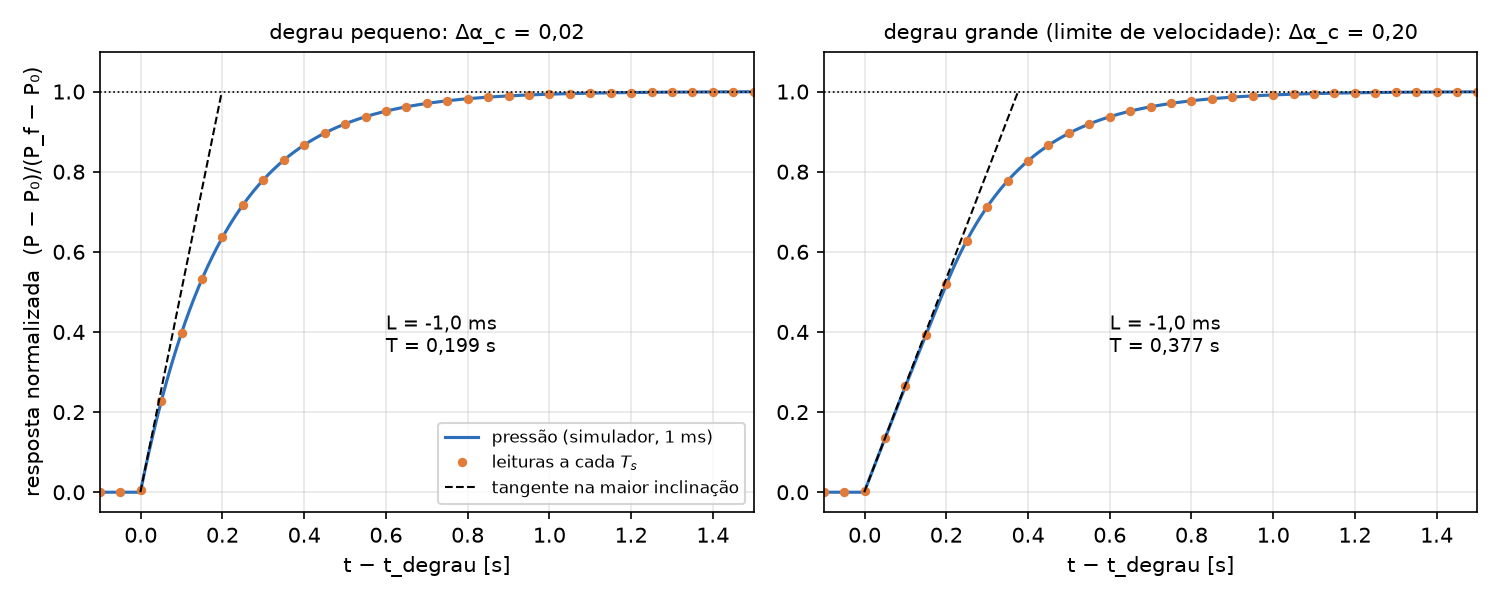
\includegraphics[width=\linewidth]{figuras/f_zn1_curva_reacao.png}
  \caption{Resposta normalizada ao degrau no comando da válvula, sete bicos. A linha azul é a
  curva do simulador (passo de 1~ms), os pontos laranja são as leituras a cada $T_s$ e a reta
  tracejada é a tangente no ponto de maior inclinação.}
\end{figure}

\begin{table}[h]
  \centering
  \begin{tabular}{lccccc}
    \toprule
    $\Delta\alpha$ & bate em $\omega_{max}$ & curva em S & $L$ & $T$ [s] & $K_g$ [kgf/cm$^2$] \\
    \midrule
    0,02 & não & não & $\approx 0$ & 0,199 & $-2{,}645$ \\
    0,20 & sim & não & $\approx 0$ & 0,377 & $-2{,}503$ \\
    \bottomrule
  \end{tabular}
\end{table}

\paragraph{Degrau pequeno.} Sem o limite de velocidade, a resposta é a de uma primeira ordem
(OGATA, 2010, p.~147):
\begin{equation}
  y(t) = 1 - e^{-(t - t_d)/\tau_a},\qquad
  \dot y(t) = \frac{1}{\tau_a}\,e^{-(t - t_d)/\tau_a}.
\end{equation}
A derivada é máxima em $t = t_d$, no próprio instante do degrau. Logo a tangente sai da origem:
\begin{equation}
  L = 0,\qquad T = \tau_a = 0{,}2\ \text{s},
\end{equation}
como o script mediu (0,199~s). A exponencial não tem ponto de inflexão, porque $\ddot y < 0$
o tempo todo.

\paragraph{Degrau grande.} A válvula anda em rampa, $\alpha - \alpha_0 = \omega_{max}(t - t_d)$,
até a velocidade pedida cair abaixo de $\omega_{max}$:
\begin{equation}
  \frac{\Delta\alpha - (\alpha - \alpha_0)}{\tau_a} = \omega_{max}
  \;\Rightarrow\; \alpha - \alpha_0 = \Delta\alpha - \omega_{max}\tau_a = 0{,}1 ,
\end{equation}
ou seja, metade do curso, em 0,2~s. Depois disso, a resposta é exponencial. A maior inclinação
continua no começo, então $L = 0$ de novo. A inclinação da rampa é cerca de
$\omega_{max}/\Delta\alpha = 2{,}5\ \text{s}^{-1}$, o que daria $T \approx 0{,}4$~s. O script
mediu 0,377~s porque $P(\alpha)$ não é linear. O $K_g$ desse degrau ($-2{,}503$) também difere
do $-2{,}66$ do TCC (Eq.~3.15), pelo mesmo motivo: aqui ele é a secante de um degrau grande, e
não a derivada no ponto de operação.

\paragraph{O $L = -1$~ms da figura.} No laço do script, a válvula já se move no mesmo passo em
que o degrau é aplicado, antes de a pressão ser calculada. Por isso $P(t_d)$ já mudou um passo,
e a tangente corta o eixo um $\Delta t$ antes. É um artefato da discretização; na prática, $L = 0$.

\paragraph{As leituras do sensor} (pontos laranja) caem em cima da curva contínua. A amostragem
não cria um atraso visível na curva de reação.

\section{E se o atraso do amostrador for usado como $L$?}

Costuma-se dizer que um controlador digital que segura o comando por um período $T_s$ equivale a
um atraso médio de $T_s/2$. Esse atraso \emph{não aparece} na curva, mas o script mostra o que
aconteceria com $L = T_s/2$ e $T = \tau_a$:
\begin{equation}
  K_c^{P} = \frac{\tau_a}{(T_s/2)\,|K_g|} = \frac{2\tau_a}{T_s\,|K_g|}
          = \frac{8}{2{,}645} = 3{,}03,\qquad
  K_c^{PI} = 2{,}72,\quad T_i = \frac{0{,}025}{0{,}3} = 0{,}083\ \text{s}.
\end{equation}

Para comparar com o limite de estabilidade do laço amostrado: com o comando parado entre duas
leituras, a válvula anda
\begin{equation}
  \alpha_{k+1} = a\,\alpha_k + (1-a)\,\alpha_{c,k},\qquad a = e^{-T_s/\tau_a} = 0{,}779 .
\end{equation}
Com o controle P, o erro passa de uma leitura para a outra multiplicado por
\begin{equation}
  e_{k+1} = \underbrace{\bigl[a - (1-a)\,K_c|K_g|\bigr]}_{z}\; e_k .
\end{equation}
Se $z$ fica entre $-1$ e $0$, o erro troca de sinal a cada leitura, mas diminui. Com
$z = -1$, a oscilação é sustentada, com período $2T_s$. Isso dá o ganho crítico:
\begin{equation}
  K_{cr} = \frac{1 + a}{(1 - a)\,|K_g|} = \frac{\coth\!\left(\dfrac{T_s}{2\tau_a}\right)}{|K_g|}
         \approx \frac{1}{|K_g|}\left(\frac{2\tau_a}{T_s} + \frac{T_s}{6\tau_a}\right) = 3{,}04 .
\end{equation}
O primeiro termo da série é exatamente o $K_c^P$ do primeiro método com $L = T_s/2$. Ou seja,
usar o atraso do amostrador põe o controlador P em $K_c^P/K_{cr} = 0{,}995$, praticamente em cima
do limite de estabilidade.

\section{Conclusão}

\begin{itemize}
  \item A resposta ao degrau é exponencial, sem forma de S, e $L = 0$. Pela condição do Ogata, o
        \textbf{1º método não se aplica}, e a Tabela 8.1 daria $K_c \to \infty$.
  \item A planta contínua, $K_g/(\tau_a s + 1)$, também não oscila com controle P, então o
        \textbf{2º método também não se aplica a rigor}. A oscilação que ele mede vem da amostragem.
  \item Forçar $L = T_s/2$ leva o P ao ganho crítico do laço amostrado. Isso reforça a proposta
        de projetar o controlador pela resposta em frequência, com margens de fase e de ganho.
\end{itemize}

\section*{Mapa função $\to$ fórmula}
\begin{tabular}{ll}
  \toprule
  Função do script & O que calcula \\
  \midrule
  \cod{degrau\_aberto} & Eqs.~(2)--(6): válvula com limite de velocidade, pressão estática, degrau em $t_d$ \\
  \cod{tangente}       & Eqs.~(8)--(10): derivada centrada, ponto de maior inclinação, $L$ e $T$ \\
  \cod{ensaio}         & Eq.~(7) e teste do S; repete o cálculo só com as leituras a cada $T_s$ \\
  \cod{tabela\_81}     & Eq.~(11): Tabela 8.1 do Ogata, dividida por $|K_g|$ \\
  \cod{main}           & os dois degraus, o caso $L = T_s/2$ (Eq.~15) e o $K_{cr}$ (Eq.~18) \\
  \bottomrule
\end{tabular}

\vspace{1em}
\small\textbf{Referências.} OGATA, K. \emph{Engenharia de controle moderno}. 5.~ed. São Paulo:
Pearson Prentice Hall, 2010. CHAPRA, S.~C.; CANALE, R.~P. \emph{Métodos numéricos para engenharia}.
5.~ed. Porto Alegre: AMGH, 2011.
\end{document}
